\chapter{Introduction}

Redaction is 'the act of removing words or information from a text before it is printed or made available to the public (Cambride Dictionary). Information or text is often redacted when it conveys sensitive information. This can be due to privacy and legal reasons, or because the text reflects the opinion of someone, or because of the risk of commercial conflicts from the publication of data. Multiple countries have \textit{Freedom of Information Acts} \cite{USAFia}, that require governmental bodies to release documents upon request of civilians. In The Netherlands the \textit{Wet open overheid (Woo)} \cite{WooWebsite} serves as such a law. This has resulted in different commercial text redaction tools in use by governments to speed up the redaction process. Different types of redacted text exist, from completely black filling (black-boxes) to gray bars to completely white, and even manual crossing out with a pen 
(\ref{fig:redactionExamples}).
\begin{figure}[h]
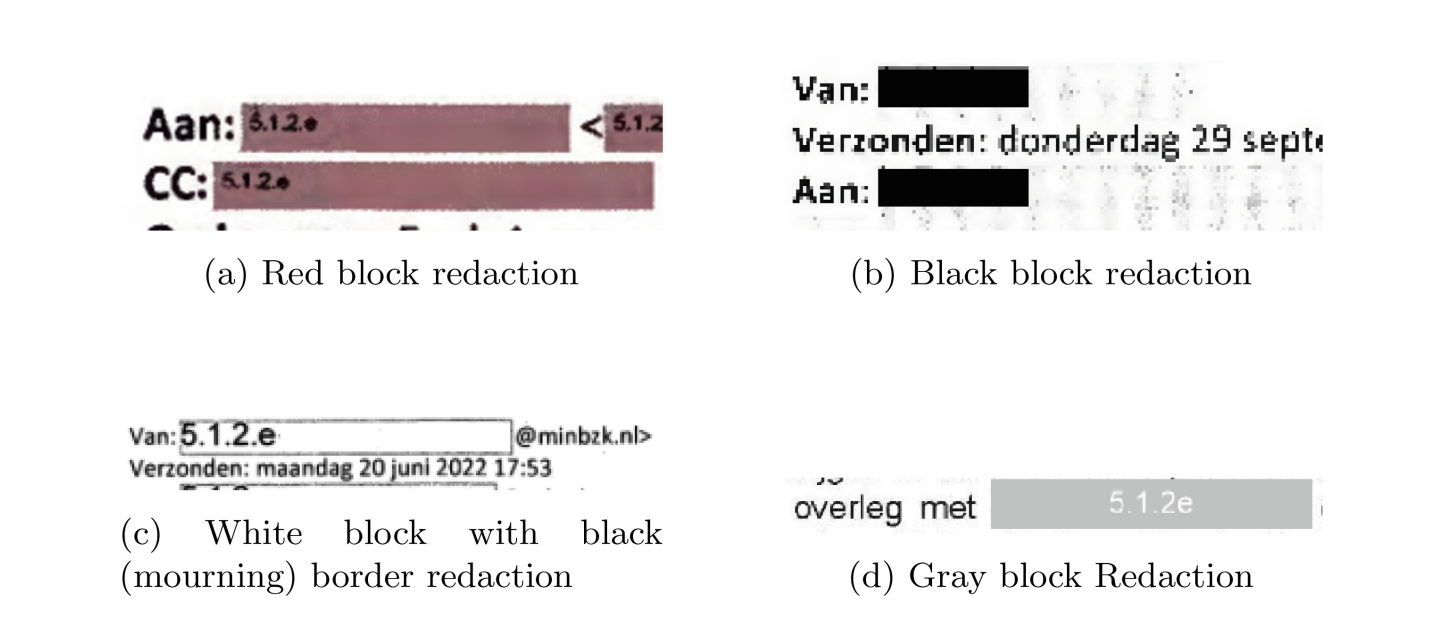
\includegraphics[width=\textwidth]{media/img.png}
\centering
\caption{Examples of four common types of text redactions. Codes like 5.1.2.e are inserted in the redacted regions to indicate the legal ground used to redact a particular piece of text.}
\label{fig:redactionExamples}
\end{figure}\\
Two essential aspects are demanded of effective redaction. First, redaction has to \textit{really} remove sensitive information from a text or document. No sensitive information should be left in the rest of the document. Secondly, the information that does not have to be redacted has to be kept intact and visible for the reader. 
\\\\
Trivial redactions \cite{forrester2005investigation}, where text is obscured visually by the use of black boxes but the underlying content remains intact, often become the subject of ridicule and mockery. There are many examples of embarrassing redaction failures \cite{failures2019} that compromise the confidentiality of  sensitive information. Besides trivial redactions, other sensitive information may still be hidden in a document after processing or redaction \cite{muller2021processing}. Advanced features such as group editing, version control and multi-user authoring leave hidden information \cite{forrester2005investigation}; versions, track changes and metadata. 
\\\\
Governments and other organisations often can not adhere to the two essential aspects of redaction due to human error or ignorance. In other instances, the focus on safety is to the detriment of the non-redacted text which is damaged; more text is redacted or non-redacted text becomes unreadable (by the computer!). In the worst case all text is removed and only images of documents are made publicly available, especially when first scanning and then again OCR-ing documents is the predominant technique used by text-redaction tools. As a result, the accessibility is greatly damaged \cite{maartenMarx} resulting in difficulties for impaired persons who want to read a document. This is often the case in the Dutch text redaction landscape. 
\\\\
\begin{figure}[h]
    \begin{subfigure}[h]{0.5\linewidth}
        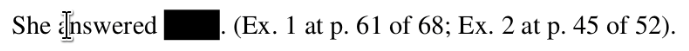
\includegraphics[width=\linewidth]{latex/media/badredaction2.png}
        \caption{A seemingly secure redaction.}
    \end{subfigure}
    \hfill
        \begin{subfigure}[h]{0.5\linewidth}
        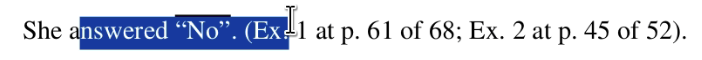
\includegraphics[width=\linewidth]{latex/media/badredaction.png}
    \caption{Selecting the box reveals the 'hidden' text.}
    \end{subfigure}%
\caption{An example of a bad redaction. The text has been 'redacted' by hiding it behind a black box. However, the actual text is not removed and hovering over it reveals the presence of the original text.}
\end{figure}\\
I present a safe PDF redaction method for documents produced with Microsoft Word that ensures confidentiality of sensitive information and does preserve non-redacted text. Redaction is done directly in the PDF which is an advantage to redaction through first scanning a document and then OCR-ing it, preserving the text and accessibility. When applicable, my method inserts placeholder text and text on the same line as a redaction is repositioned. Furthermore, hidden information is either deleted or changed when possible. Finally, noise is added to positional information of glyphs in order to make it computationally more difficult to determine what the redacted text was. For non-Word documents, partial or complete confidentiality after redaction may be ensured depending on the workflow used to generate the PDF.
\\\\
I was able to validate my redaction method using both custom made documents of various complexity and real-world examples made publicly available by governmental bodies in the Netherlands. I was able to prove that for most cases, safe redaction can be performed. \textbf{to be added...}
\\\\


%## Onderzoeksvragen
%
%-  How can text redaction be accomplished directly in PDF documents while ensuring that redacted text can not be %retrieved back in any way and preserving the accessibility by not damaging or changing the non-redacted text in %any way?
%
%    1. What is text redaction and how is it used?
%        1. What is the redaction of text?
%        2. In what context (or contexts) is text redaction used?
%        3. What type of redactions can be found in publicly available documents?
%        4. What essential principles are demanded of effective redaction to ensure safety and preservation?
%        5. What are the most common text redaction software used by governmental bodies in the Netherlands and %how do they redact text?
%     2. What are concerns related to text redaction in PDF?
%        1. How may security of text redaction be compromised by human error or ignorance?
%        2. How may the accessibility of a document be damaged as a result of redaction?
%        3. Are there any advanced techniques which may compromise the security of a text redaction?
%        4. Are there any tools which detect and/or fix bad redactions?
%     3. What is an effective approach to text redaction in PDF documents that adheres to the two principles and %what are the challenges?
%         1. How may to-be-redacted text be represented in a PDF document and where may it be found within the %document?
%         2. How may to-be-redacted text be labelled and located in a PDF?
%         3. How might text be removed from a PDF to ensure that it is really removed from the document?
%         4. What should be done with positional information after redaction and is it possible to find a balance %between security and accessibility?
%         5. How may white spaces as a result of redaction be removed?
%         6. What kind(s) of metadata might there be in a document and how might they be checked to ensure safe redaction?
 %    7. How can an effective redaction approach be implemented?
 %        1. Are there any publicly available means where can be built upon and what should I add upon these to %realise an effective approach?
 %        2. What steps can be defined when creating a text redaction algorithm and what are the relevant aspects and difficulties of each step?
 %        3. What are the practical limitations (document type support, white space removal, metadata) and how might they be solved theoretically? 
%   8. How can an effective approach be validated?
%         1. How should the input of the redaction algorithm be compared to the output to validate the algorithm?
%         2. What type of documents should be experimented on and what are some sources that might be used for %these documents? What corpus can be constructed?
%     9. Based on this research and its findings, what are recommendations and considerations for practical text %redaction in PDF, and further research in the field?
  



